\chapter{DEPLOYMENT}

\section{Folder Structure}

\begin{figure}[H]
    \centering
    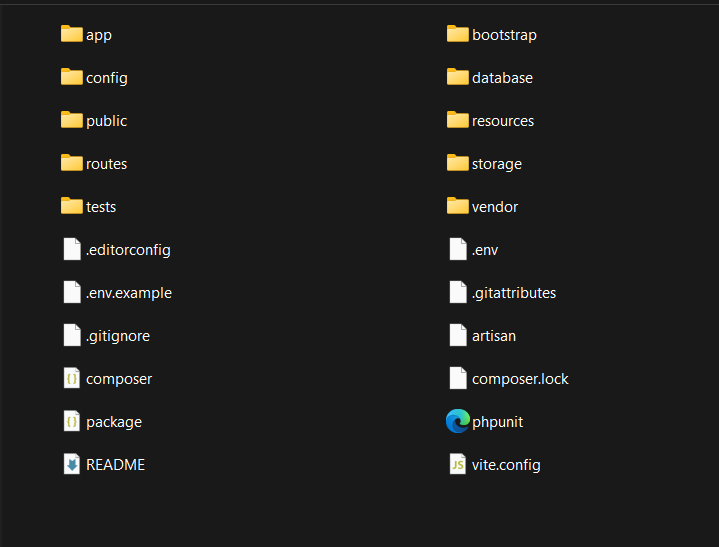
\includegraphics[width=0.8\textwidth]{Screenshot 2026-03-02 014217.png}
    \caption{Project files and important folders}
    \label{fig:Use_case}
\end{figure}

The Medora Hospital Management System follows the standard Laravel project structure, which ensures modularity, maintainability, and scalability. The folder structure is organized in a way that separates business logic, views, configurations, and database management.

\subsection*{Main Project Directories}

\textbf{app/}  
This directory contains the core application logic. It includes:
\begin{itemize}
    \item Models (User, Doctor, Patient, Appointment, Prescription, LabTest, Billing, Medicine, etc.)
    \item Controllers that handle request processing and business logic
    \item Middleware for role-based access control and authentication
\end{itemize}

\textbf{routes/}  
Contains route definitions for web and API requests. The \texttt{web.php} file manages system routing between pages and controllers.

\textbf{resources/}  
Includes frontend components such as:
\begin{itemize}
    \item Blade view files for dashboards and forms
    \item CSS and JavaScript assets
\end{itemize}

\textbf{database/}  
Contains:
\begin{itemize}
    \item Migration files for creating database tables
    \item Seeders for inserting default data
\end{itemize}

\textbf{public/}  
This is the publicly accessible directory that contains:
\begin{itemize}
    \item Index file (entry point of the application)
    \item Uploaded files such as prescriptions and lab reports
    \item Public assets
\end{itemize}

\textbf{storage/}  
Stores generated files, logs, and uploaded documents securely.

\textbf{config/}  
Contains configuration settings for database connection, authentication, mail services, and application settings.

\subsection*{Deployment Process}

To deploy the system:

\begin{itemize}
    \item Install required dependencies using Composer.
    \item Configure the environment file (.env) with database credentials.
    \item Run database migrations to create required tables.
    \item Start the Apache/Nginx server.
    \item Access the system through the configured domain or localhost.
\end{itemize}

The structured folder organization ensures that the system is easy to deploy, maintain, and extend in future updates.